\documentclass[12pt]{article}

\usepackage[margin=1in]{geometry}
\usepackage{amsmath,amssymb}
\usepackage{algorithm}
\usepackage{algorithmic}
\usepackage{booktabs}
\usepackage{graphicx}

%% Rename the default labels for \REQUIRE and \ENSURE
\renewcommand{\algorithmicrequire}{\textbf{Input:}}
\renewcommand{\algorithmicensure}{\textbf{Output:}}

\begin{document}

\section{Empirical Results}

\begin{figure}[htp!]
    \centering
    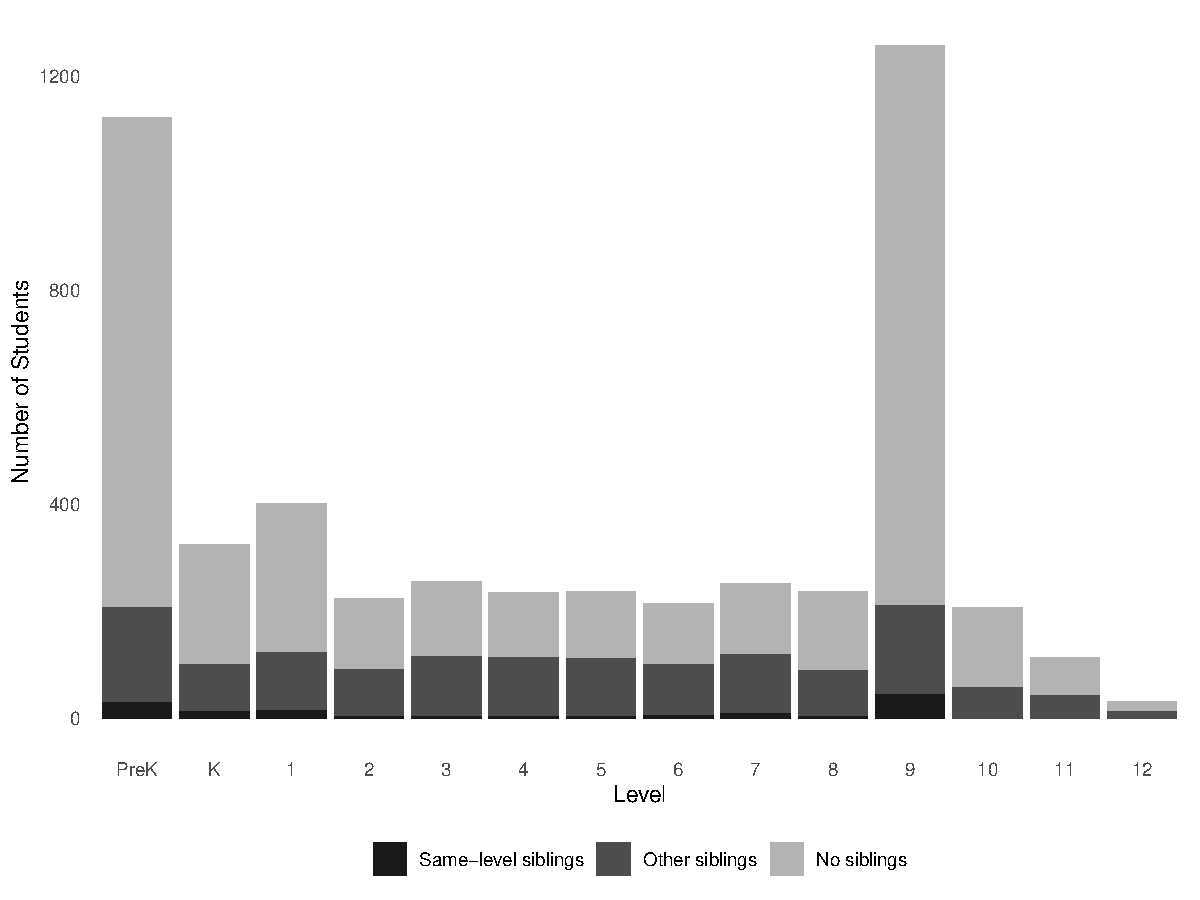
\includegraphics[width=\textwidth]{../plots/distribution_applicants_per_level_Magallanes_2023.pdf}
    \caption{Summary Statistics by Region, Admissions Process 2023-2024}
\end{figure}

\begin{table}[htp!]
    \caption{\label{tab:general summary stats}Summary Statistics by Region, Admissions Process 2023-2024}
    \centering
    \begin{tabular}[t]{lccccccccc}
        \toprule
        \multicolumn{5}{c}{ } & \multicolumn{5}{c}{Siblings}                                                                                                                                                        \\
        \cmidrule(l{3pt}r{3pt}){6-10}
        \multicolumn{1}{c}{ } & \multicolumn{2}{c}{Schools}  & \multicolumn{2}{c}{Students} & \multicolumn{1}{c}{Pairs} & \multicolumn{2}{c}{Same Level} & \multicolumn{2}{c}{Block}                                \\
        \cmidrule(l{3pt}r{3pt}){2-3} \cmidrule(l{3pt}r{3pt}){4-5} \cmidrule(l{3pt}r{3pt}){6-6} \cmidrule(l{3pt}r{3pt}){7-8} \cmidrule(l{3pt}r{3pt}){9-10}
        Region                & N                            & Seats                        & N                         & Applications                   & N                         & N    & \%    & N     & \%    \\
        \midrule
        Tarapaca              & 1345                         & 18653                        & 16577                     & 56613                          & 3929                      & 189  & 0.048 & 2005  & 0.510 \\
        Antofagasta           & 1477                         & 28428                        & 24335                     & 86855                          & 4299                      & 283  & 0.066 & 2138  & 0.497 \\
        Atacama               & 1189                         & 20603                        & 11910                     & 37910                          & 1991                      & 143  & 0.072 & 899   & 0.452 \\
        Coquimbo              & 4800                         & 54033                        & 27892                     & 101412                         & 5345                      & 347  & 0.065 & 2934  & 0.549 \\
        Valparaíso            & 8476                         & 111273                       & 52747                     & 170340                         & 9202                      & 660  & 0.072 & 5340  & 0.580 \\
        OHiggins              & 4908                         & 67203                        & 30752                     & 93230                          & 4592                      & 407  & 0.089 & 2387  & 0.520 \\
        Maule                 & 6281                         & 80627                        & 35607                     & 116467                         & 5340                      & 438  & 0.082 & 2636  & 0.494 \\
        Biobio                & 7466                         & 110395                       & 46596                     & 156956                         & 7352                      & 544  & 0.074 & 3957  & 0.538 \\
        Araucania             & 8105                         & 91032                        & 31930                     & 91032                          & 4349                      & 332  & 0.076 & 2161  & 0.497 \\
        Lagos                 & 6590                         & 73535                        & 27054                     & 85040                          & 4211                      & 277  & 0.066 & 2259  & 0.536 \\
        Aysen                 & 721                          & 9330                         & 3293                      & 8886                           & 461                       & 33   & 0.072 & 232   & 0.503 \\
        Magallanes            & 671                          & 9540                         & 5113                      & 16035                          & 807                       & 68   & 0.084 & 443   & 0.549 \\
        Metropolitana         & 20063                        & 357793                       & 200539                    & 726155                         & 34903                     & 2275 & 0.065 & 19886 & 0.570 \\
        Rios                  & 3240                         & 38175                        & 12505                     & 34465                          & 1757                      & 137  & 0.078 & 838   & 0.477 \\
        Arica                 & 919                          & 13169                        & 7566                      & 24401                          & 1251                      & 80   & 0.064 & 767   & 0.613 \\
        Nuble                 & 3349                         & 43759                        & 14461                     & 41824                          & 1928                      & 152  & 0.079 & 1065  & 0.552 \\
        Overall               & 79600                        & 1127548                      & 536353                    & 1847621                        & 91717                     & 6365 & 0.069 & 49947 & 0.545 \\
        \bottomrule
    \end{tabular}
\end{table}

\clearpage
\section{Simultaneous Algorithm}

We present the pseudocode for the \emph{Simultaneous} heuristic. The algorithm
takes as input a matching instance consisting of: a finite set of students
$S$; a finite set of schools $C$, where each school $c\in C$ offers
$q_c^\ell \in \mathbb{Z}_+$ seats at level $\ell\in L$ (with $q_c^\ell = 0$
meaning school $c$ does not offer level $\ell$); a family partition
$\mathcal{F}\subseteq 2^S$ of $S$, where $f(s)\in\mathcal{F}$ denotes the
family of student $s\in S$; strict student preferences
$(\succ_s)_{s\in S}$ over $C\cup\{\emptyset\}$; and initial school
priority orders $(\succ_c)_{c\in C}$ over $S$, derived from group
mappings $g(s,c)$ and random tie-breakers $(p_{s,c})_{s\in S,\,c\in C}$. The
set of feasible student--school pairs is
\[
    V \;=\; \{(s,c)\in S\times C : c\succ_s\emptyset,\; q_c^{\ell(s)}>0\},
\]
where $\ell(s)$ denotes the level of student $s$.

Unlike the Descending benchmark, which processes levels sequentially from
highest to lowest, the Simultaneous algorithm runs the student-proposing
Deferred Acceptance (DA) algorithm over \emph{all} students at once. After
each run of DA, it updates the priority orders by promoting, to the top of the
queue, any student $s'$ whose sibling has just been matched to the same school.
Specifically, if student $s$ is assigned to school $c$, then for every sibling
$s'\in f(s)\setminus\{s\}$ who also applies to $c$, student $s'$ is elevated in
$c$'s priority ranking. This update is \emph{monotone}: once a student gains
elevated priority at a school, that status is preserved in all subsequent
iterations regardless of later changes to the matching. The process repeats
until the matching stabilises, i.e., no student changes their assignment between
two consecutive iterations.

\bigskip

\begin{algorithm}[H]
    \caption{Simultaneous}
    \label{alg:simultaneous}
    \begin{algorithmic}[1]
        \REQUIRE Matching instance
        $\bigl(S,\,C,\,\mathcal{F},\,(\succ_s)_{s\in S},\,(\succ_c)_{c\in C},\,(q_c^\ell)_{c\in C,\,\ell\in L}\bigr)$
        \ENSURE Matching $\mu^t$

        \STATE Set $z_{s,c} \leftarrow 0$ for all $s\in S$, $c\in C$
        \COMMENT{no sibling priority initially}
        \STATE Set $\succ_c^{0} \leftarrow \succ_c$ for all $c\in C$
        \COMMENT{start from initial priority orders}
        \STATE Set $t \leftarrow 0$

        \LOOP

        \STATE Compute $\mu^{t} \;\leftarrow\;
            \mathrm{DA}\!\left(
            S,\;
            (\succ_s)_{s\in S},\;
            (\succ_c^{t})_{c\in C},\;
            (q_c^\ell)_{c\in C,\,\ell\in L}
            \right)$

        \IF{$t \;\geq\; 1$
            \AND
            $\mu^{t}(s) = \mu^{t-1}(s)$ for all $s\in S$}
        \STATE \textbf{break} \COMMENT{matching has converged}
        \ENDIF

        \FOR{each $s\in S$ such that $\mu^{t}(s)\neq\emptyset$}
        \FOR{each $s'\in f(s)\setminus\{s\}$}
        \STATE Set $z_{s',\,\mu^{t}(s)} \leftarrow 1$
        \COMMENT{$s'$ receives sibling priority at school $\mu^t(s)$}
        \ENDFOR
        \ENDFOR

        \FOR{each $c\in C$}
        \STATE Update $\succ_c^{t+1}$: students $s$ with $z_{s,c}=1$ precede
        those with $z_{s,c}=0$; ties within each group are broken using
        $\succ_c$
        \ENDFOR

        \STATE Set $t \leftarrow t+1$

        \ENDLOOP

        \RETURN $\mu^{t}$

    \end{algorithmic}
\end{algorithm}

\bigskip

\paragraph{Notes.}
\begin{itemize}
    \item $\mathrm{DA}$ denotes the student-proposing Deferred Acceptance
          algorithm (Gale and Shapley 1962). Given school priority orders
          $(\succ_c^t)_{c\in C}$ and capacities $(q_c^\ell)$, it returns the
          student-optimal stable matching with respect to those priorities.
    \item The variables $z_{s,c}\in\{0,1\}$ track cumulative sibling
          priority: $z_{s,c}=1$ means that at some iteration $\tau\leq t$ a sibling
          of $s$ was matched to school~$c$, and this status is never revoked. If sibling priorities are reset at the beginning of each iteration based on the current assignment, the algorithm may fail to converge, as students can repeatedly gain and lose priority at the same school across iterations.
    \item The priority update in lines 9--12 implements \emph{absolute}
          contingent priority (Definition~3 in the paper): any student whose sibling
          has been matched to school $c$ is placed in a strictly higher priority tier
          than students with no sibling matched to $c$, with ties within each tier
          broken by the initial order~$\succ_c$.
    \item The algorithm terminates when two consecutive matchings coincide.
          Convergence is guaranteed in finite time because $|S|$ and $|C|$ are finite
          and the sibling-priority indicator $z_{s,c}$ is monotone
          non-decreasing, so the set of priority-elevated students can only grow (or
          stay the same) between iterations.
\end{itemize}


Another algorithm that we can consider is DA + Improvement Cycles.

\end{document}
